% 12 variables in here:
% u_1 = 0.0, h_1 = 10.0, U_1 = 0.0, H_1 = 10.0, u_2 = 0.0, h_2 = 10.0, U_2 = 0.0, H_2 = 10.0, u_3 = 0.0, h_3 = 10.0, U_3 = 0.0, H_3 = 10.0
\begin{figure}[h!t]
\centering
  \subfigure[Impulse error of $p_1^L$, $p_1^R$, $p_3^L$ resp. $p_3^R$ for equidistant support points at $\{0, \frac{1}{2}, 1\}$] {
    %\includegraphics[scale=\zoomfactor]{{{3_punkte_equidist_alles_gleich/x_y_0.0_10.0_0.0_10.0_0.0_10.0_0.0_10.0_0.0_10.0f0}}}  
    \begin{tikzpicture}
      \node at (0,0) {\includegraphics[scale=\zoomfactor]{{{3_punkte_equidist_alles_gleich/x_y_0.0_10.0_0.0_10.0_0.0_10.0_0.0_10.0_0.0_10.0f1}}}  };
      \fill[white] (.8,1.2) rectangle (1.75,1.5);
      \node[align=right, text width=3cm] at (.2,1.33) {\textsf{\tiny{Impulse error}}};
    \end{tikzpicture}
  }
  \hspace{.3cm}
  \subfigure[Impulse error of $p_2^L$ resp. $p_2^R$ for equidistant support points at $\{0, \frac{1}{2}, 1\}$] {
    %\includegraphics[scale=\zoomfactor]{{{3_punkte_equidist_alles_gleich/0.0_10.0_0.0_10.0_x_y_0.0_10.0_0.0_10.0_0.0_10.0f0}}}  
    \begin{tikzpicture}
      \node at (0,0) {\includegraphics[scale=\zoomfactor]{{{3_punkte_equidist_alles_gleich/0.0_10.0_0.0_10.0_x_y_0.0_10.0_0.0_10.0_0.0_10.0f1}}}  };
      \fill[white] (.8,1.2) rectangle (1.75,1.5);
      \node[align=right, text width=3cm] at (.2,1.33) {\textsf{\tiny{Impulse error}}};
    \end{tikzpicture}
  }
  % \subfigure[Height and impulse of $p_3^L$ resp. $p_3^R$.] {
  %   %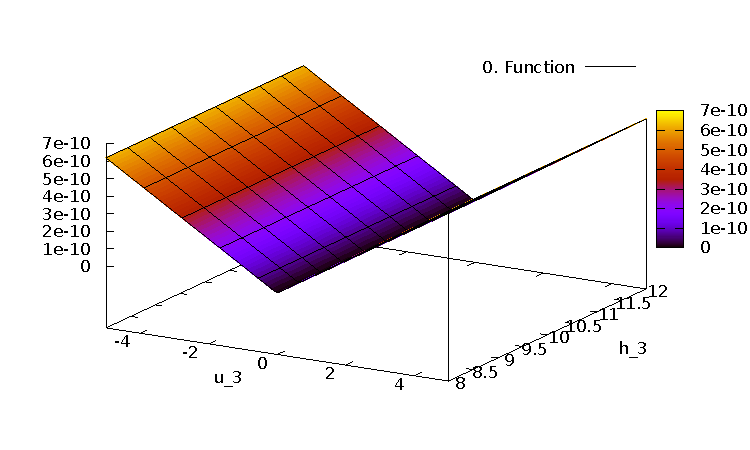
\includegraphics[scale=\zoomfactor]{{{3_punkte_equidist_alles_gleich/0.0_10.0_0.0_10.0_0.0_10.0_0.0_10.0_x_y_0.0_10.0f0}}}  
  %   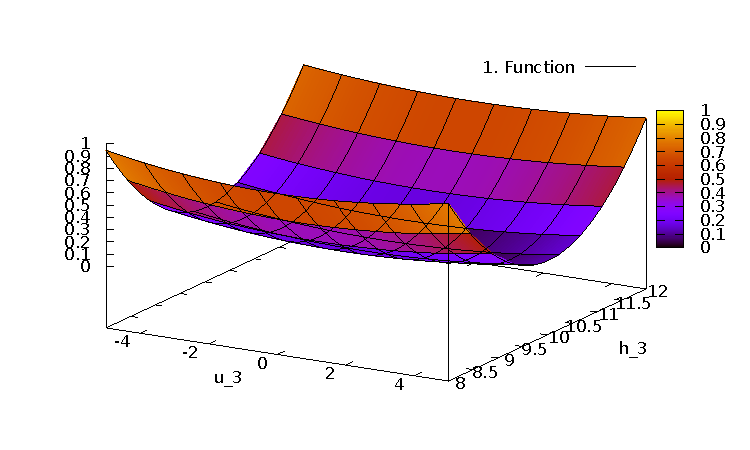
\includegraphics[scale=\zoomfactor]{{{3_punkte_equidist_alles_gleich/0.0_10.0_0.0_10.0_0.0_10.0_0.0_10.0_x_y_0.0_10.0f1}}}  
  % }
  % \subfigure[Height and impulse of $p_1^R$.] {
  %   %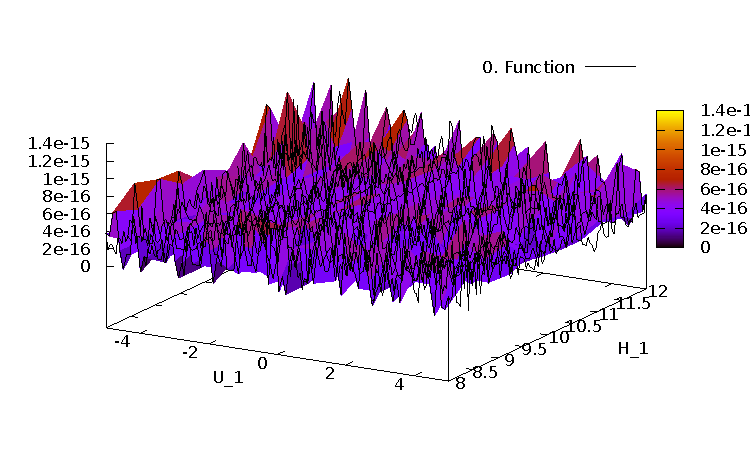
\includegraphics[scale=\zoomfactor]{{{3_punkte_equidist_alles_gleich/0.0_10.0_x_y_0.0_10.0_0.0_10.0_0.0_10.0_0.0_10.0f0}}}  
  %   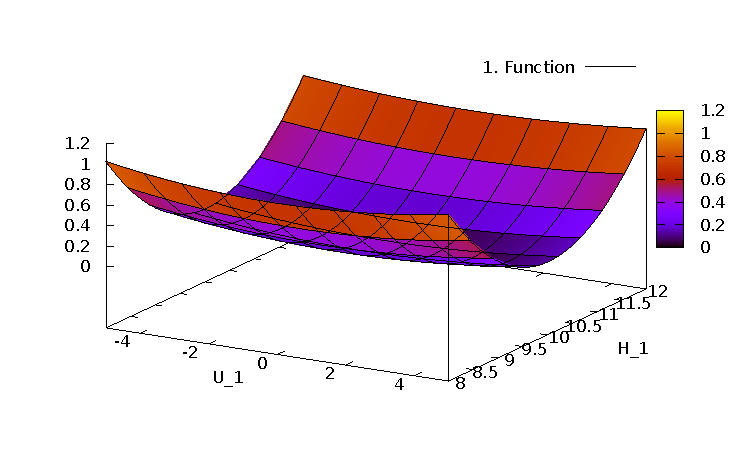
\includegraphics[scale=\zoomfactor]{{{3_punkte_equidist_alles_gleich/0.0_10.0_x_y_0.0_10.0_0.0_10.0_0.0_10.0_0.0_10.0f1}}}  
  % }
  % \subfigure[Height and impulse of $p_2^R$.] {
  %   %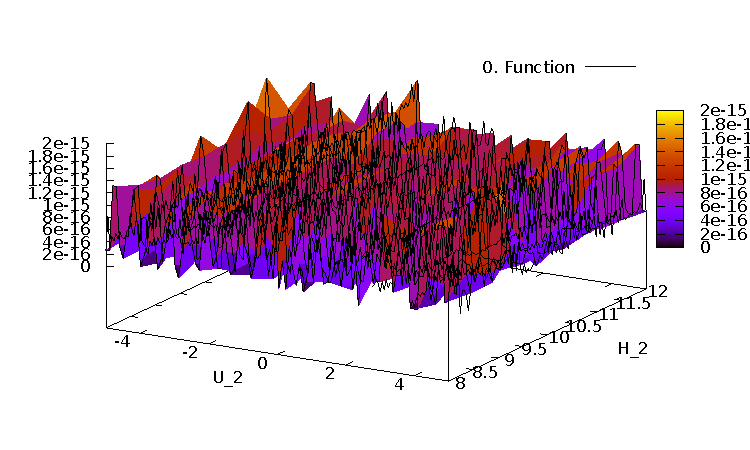
\includegraphics[scale=\zoomfactor]{{{3_punkte_equidist_alles_gleich/0.0_10.0_0.0_10.0_0.0_10.0_x_y_0.0_10.0_0.0_10.0f0}}}  
  %   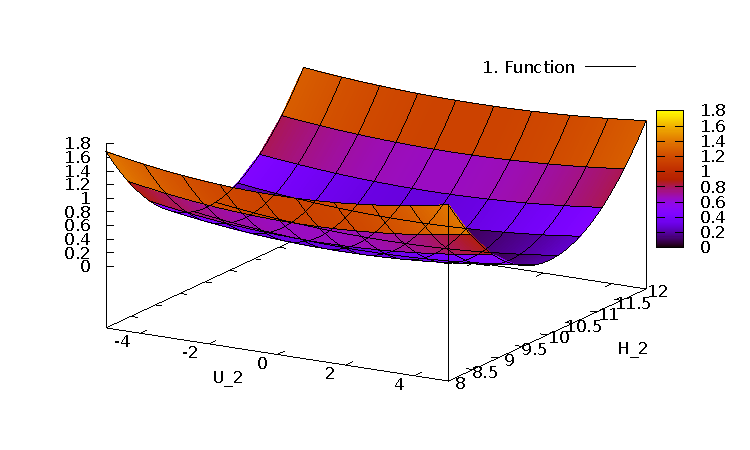
\includegraphics[scale=\zoomfactor]{{{3_punkte_equidist_alles_gleich/0.0_10.0_0.0_10.0_0.0_10.0_x_y_0.0_10.0_0.0_10.0f1}}}  
  % }
  % \subfigure[Height and impulse of $p_3^R$.] {
  %   %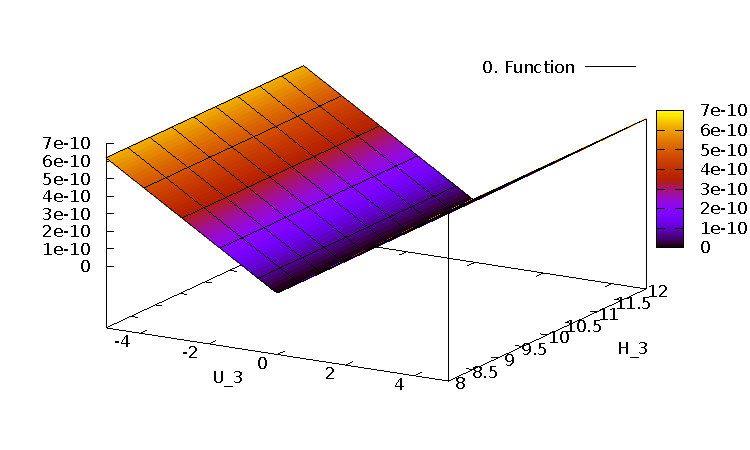
\includegraphics[scale=\zoomfactor]{{{3_punkte_equidist_alles_gleich/0.0_10.0_0.0_10.0_0.0_10.0_0.0_10.0_0.0_10.0_x_yf0}}}  
  %   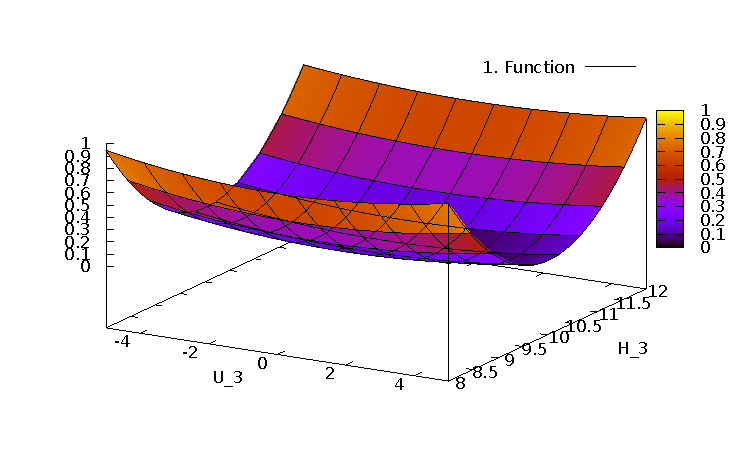
\includegraphics[scale=\zoomfactor]{{{3_punkte_equidist_alles_gleich/0.0_10.0_0.0_10.0_0.0_10.0_0.0_10.0_0.0_10.0_x_yf1}}}  
  % }

  \subfigure[Impulse error for point $p_1^L$, $p_3^L$, $p_1^R$ resp. $p_3^R$ for support points at $\{-\frac{\sqrt{15}}{10}\pm\frac{1}{2}, 0\}$] {
    % \begin{tikzpicture}
    %   \node at (0,0) {\includegraphics[scale=\zoomfactor]{{{3_punkte_gleich/x_y_0.0_10.0_0.0_10.0_0.0_10.0_0.0_10.0_0.0_10.0f0}}}   };
    %   \fill[white] (.8,1.2) rectangle (1.75,1.5);
    %   \node[align=right, text width=3cm] at (.2,1.33) {\textsf{\tiny{Height error}}};
    % \end{tikzpicture}
    \begin{tikzpicture}
      \node at (0,0) {\includegraphics[scale=\zoomfactor]{{{3_punkte_gleich/x_y_0.0_10.0_0.0_10.0_0.0_10.0_0.0_10.0_0.0_10.0f1}}}   };
      \fill[white] (.8,1.2) rectangle (1.75,1.5);
      \node[align=right, text width=3cm] at (.2,1.33) {\textsf{\tiny{Impulse error}}};
    \end{tikzpicture}
  }
  \hspace{.3cm}
  \subfigure[Impulse error for point $p_2^L$ resp. $p_2^R$ for support points at $\{-\frac{\sqrt{15}}{10}\pm\frac{1}{2}, 0\}$] {
    % \begin{tikzpicture}
    %   \node at (0,0) {\includegraphics[scale=\zoomfactor]{{{3_punkte_gleich/0.0_10.0_0.0_10.0_x_y_0.0_10.0_0.0_10.0_0.0_10.0f0}}}   };
    %   \fill[white] (.8,1.2) rectangle (1.75,1.5);
    %   \node[align=right, text width=3cm] at (.2,1.33) {\textsf{\tiny{Height error}}};
    % \end{tikzpicture}
    \begin{tikzpicture}
      \node at (0,0) {\includegraphics[scale=\zoomfactor]{{{3_punkte_gleich/0.0_10.0_0.0_10.0_x_y_0.0_10.0_0.0_10.0_0.0_10.0f1}}}   };
      \fill[white] (.8,1.2) rectangle (1.75,1.5);
      \node[align=right, text width=3cm] at (.2,1.33) {\textsf{\tiny{Impulse error}}};
    \end{tikzpicture}
  }
\caption{Three support points. Coordinates of points are $(10,0)^T$. We compare equidistant support points to support points obtained from Gaussian quadrature.}
\label{fig:three-equidistant-all-fixed}
\end{figure}

%%% Local Variables:
%%% TeX-master: "../results.tex"
%%% End:

%%% Local Variables:
%%% TeX-master: "../results.tex"
%%% End:
